\documentclass[11pt,]{article}
% \setcounter{tocdepth}{5}
% \setcounter{secnumdepth}{5}

\usepackage{hyperref}
\usepackage[T1]{fontenc}
\usepackage{amssymb,amsmath}
\usepackage{txfonts}
\usepackage{microtype}
\usepackage{amssymb,amsmath}
\usepackage{graphicx}
\usepackage{subfig} 
\usepackage{natbib}
\usepackage{paralist}
\usepackage{hyperref}
\usepackage{url}
\urlstyle{same}
\usepackage{color}
\usepackage{fancyvrb}
\usepackage[a4paper,body={170mm,250mm},top=25mm,left=25mm,head=14pt]{geometry}
\usepackage{fancyhdr}
\usepackage{xspace}
\xspaceaddexceptions{\%}
\renewcommand*\ttdefault{txtt} % 20% tighter than courier

%% uses fancyvrb
\newcommand{\VerbBar}{|}
\newcommand{\VERB}{\Verb[commandchars=\\\{\}]}
\DefineVerbatimEnvironment{Highlighting}{Verbatim}{commandchars=\\\{\}}
% Add ',fontsize=\small' for more characters per line

\newenvironment{Shaded}{}{}
\newcommand{\KeywordTok}[1]{\textcolor[rgb]{0.00,0.44,0.13}{\textbf{{#1}}}}
\newcommand{\DataTypeTok}[1]{\textcolor[rgb]{0.56,0.13,0.00}{{#1}}}
\newcommand{\DecValTok}[1]{\textcolor[rgb]{0.25,0.63,0.44}{{#1}}}
\newcommand{\BaseNTok}[1]{\textcolor[rgb]{0.25,0.63,0.44}{{#1}}}
\newcommand{\FloatTok}[1]{\textcolor[rgb]{0.25,0.63,0.44}{{#1}}}
\newcommand{\CharTok}[1]{\textcolor[rgb]{0.25,0.44,0.63}{{#1}}}
\newcommand{\StringTok}[1]{\textcolor[rgb]{0.25,0.44,0.63}{{#1}}}
\newcommand{\CommentTok}[1]{\textcolor[rgb]{0.38,0.63,0.69}{\textit{{#1}}}}
\newcommand{\OtherTok}[1]{\textcolor[rgb]{0.00,0.44,0.13}{{#1}}}
\newcommand{\AlertTok}[1]{\textcolor[rgb]{1.00,0.00,0.00}{\textbf{{#1}}}}
\newcommand{\FunctionTok}[1]{\textcolor[rgb]{0.02,0.16,0.49}{{#1}}}
\newcommand{\RegionMarkerTok}[1]{{#1}}
\newcommand{\ErrorTok}[1]{\textcolor[rgb]{1.00,0.00,0.00}{\textbf{{#1}}}}
\newcommand{\NormalTok}[1]{{#1}}

\hypersetup{breaklinks=true,
            pdfauthor={},
            pdftitle={},
            colorlinks=true,
            citecolor=blue,
            urlcolor=blue,
            linkcolor=magenta,
            pdfborder={0 0 0}}

\setlength{\parindent}{0pt}
\setlength{\parskip}{6pt plus 2pt minus 1pt}
\setlength{\emergencystretch}{3em}  % prevent overfull lines

\newcommand{\todo}[2]{{\textcolor{red}{\bf [#1] #2 }}\addcontentsline{toc}{subsubsection}{\textcolor{red}{[#1] #2} }}
\newcommand{\notes}[1]{\textcolor{blue}{\it #1 }}

\DeclareMathOperator{\softmax}{softmax}
\DeclareMathOperator{\sigmoid}{sigmoid}
\DeclareMathOperator{\sgn}{sgn}
\DeclareMathOperator{\relu}{relu}
\DeclareMathOperator{\lrelu}{lrelu}
\DeclareMathOperator{\elu}{elu}
\DeclareMathOperator{\selu}{selu}
\DeclareMathOperator{\maxout}{maxout}


%% uses fancyhdr
\pagestyle{fancy}

\author{}
\date{}


\usepackage{cleveref}

%% uses fancyhdr
\usepackage{titlesec}
\lhead{\sffamily MLP 2020/21:  Coursework 2}
\rhead{\sffamily Due: 30 November 2020}
\cfoot{\sffamily \thepage}
\crefformat{footnote}{#2\footnotemark[#1]#3}
\usepackage{dirtree}

\def\pagelimit{6\xspace}
\def\markweight{40\xspace}

\begin{document}

\begin{center}
\textsf{\textbf{\Large Machine Learning Practical 2020/21: Coursework 2}}

\bigskip
\textbf{Released: Monday 16 November 2020}

\textbf{Submission due: 16:00 Monday 30 November 2020 (extended from 27th)}
\end{center}
\section{Introduction}
\label{sec:introduction}

The aim of this coursework is to explore the classification of images using convolutional neural networks on a different dataset, \href{https://www.cs.toronto.edu/~kriz/cifar.html}{CIFAR100} (pronounced as ``see far 100''). CIFAR100 consists of 60,000 $32 \times 32$ colour images in 100 classes, with 600 images per class. The first part of the coursework concerns with debugging a ``broken'' neural network and quantitatively analyzing the problem behind this broken network. The second part involves exploring the solutions in literature for fixing this ``broken'' neural network, and then subsequently implementing one of these solutions to improve the performance and training of this network. 

In order to support your experiments, we have acquired Google Cloud Platform credits which allow the use of the  \href{https://cloud.google.com/compute/docs/}{Google Compute Engine} infrastructure.
You will need this to run all the tasks of the coursework (which will be carried out in \href{https://pytorch.org}{PyTorch}). Each student enrolled on the MLP course will receive a \$50 Google Cloud credit coupon which is enough to carry out the experiments required for this coursework. You will receive an email which will give you the URL you will need to access in order to request your Google Cloud Platform coupon. 

As in the previous coursework, you will need to submit your python code and a report. The detailed submission instructions are given in Section \ref{sec:submission} -- please follow these instructions carefully.

\section{Github branch \texttt{mlp2020-21/coursework\_2}}
\label{sec:code}

The provided code and setup information for this coursework is available on the course
\href{https://github.com/VICO-UoE/mlpractical}{Github repository}
on a branch \verb+mlp2020-21/coursework_2+. To create a local working
copy of this branch in your local repository you need to do the
following.

\begin{enumerate}
% \def\labelenumi{\arabic{enumi}.}
% \itemsep3pt\parskip0pt\parsep0pt
\item
  Make sure all modified files on the branch you are currently have been
  committed
  (see \href{https://github.com/VICO-UoE/mlpractical/blob/mlp2020-21/lab7/notes/getting-started-in-a-lab.md}{notes/getting-started-in-a-lab.md} if you are unsure how to do this).
\item
  Fetch changes to the upstream \texttt{origin} repository by running\\
  \texttt{git fetch origin}
\item
  Checkout a new local branch from the fetched branch using\\
  \verb+git checkout -b coursework_2 origin/mlp2020-21/coursework_2+
\end{enumerate}

You will now have a new branch in your local repository with everything you need to carry out the coursework.

Before continuing, remember to run \texttt{bash install.sh} to install some additional dependencies required. This assumes that you have already installed your environment as explained in \textbf{Lab1}, under \texttt{notes/environment-set-up.md}.

This branch includes the following additions to your setup:

\begin{itemize}
    \item For the PyTorch Framework: 
    \begin{itemize}
        \item A Jupyter notebook, \texttt{Coursework\_2\_Pytorch\_Introduction.ipynb}, which introduces Pytorch, and provides further resources on tutorials, documentation and debugging.
        \item A directory \texttt{pytorch\_mlp\_framework/}, which includes tooling and ready to run scripts to enable straightforward experimentation on GPU.  Documentation on this is included in  \texttt{notes/pytorch-experiment-framework.md}
        \item A note on how to use the Google Cloud Platform (using your student credits),\\\texttt{notes/google\_cloud\_setup.md}.
    \end{itemize}
     \item For the report:
    \begin{itemize}
        \item  A directory called  \texttt{report} which contains the LaTeX template and style files for your report.  You should copy all these files into the directory which will contain your report.
    \end{itemize}
\end{itemize}


\section{Tasks}
\label{sec:tasks}

This coursework has three tasks and objectives: 
\begin{itemize}
    \item Diagnose a deep CNN that cannot be properly trained due to optimization issues. Discuss what the problem is, why it happens in a deep CNN and quantitatively analyze the problem. 
    \item Discuss solutions present in the literature to address this problem.  
    \item Propose in detail and implement one of the solutions to the problem. Since the aim of this is to improve the \texttt{training} behaviour of the network, the solutions should then be evaluated in terms of {convergence speed} and {per-epoch training accuracy/loss} and {gradient flows}.
\end{itemize}

Carrying out larger convolutional network experiments using the MLP numpy framework is computationally inefficient because (1) it runs on CPU and not on GPU, and (2) a  default implementation of a convolutional layer is unlikely to be computationally efficient. For these reasons in this coursework, which involves running convolutional network experiments we will use GPU computing (on the Google Compute Engine) and the highly efficient PyTorch framework.



\section{Task 1: Identifying training problems of a deep CNN}
\label{sec:pytorch}
\textit{Time budget\footnote{\label{footnote:time-budget} These are simply suggested guidelines, feel free to adjust them based on your own preferences}: This section should take about 20\% of the time you have allocated for your coursework.}\newline

This part of the coursework involves debugging and tuning deep CNNs using PyTorch and the Google Compute Engine.

Identifying and resolving any optimization-related problems that might prevent your model from fitting the training set are critical skills when working with deep neural networks. Being able to work around this problem is key to building high performance deep neural networks.

\begin{figure}
\centering
\begin{minipage}{.5\textwidth}
  \centering
  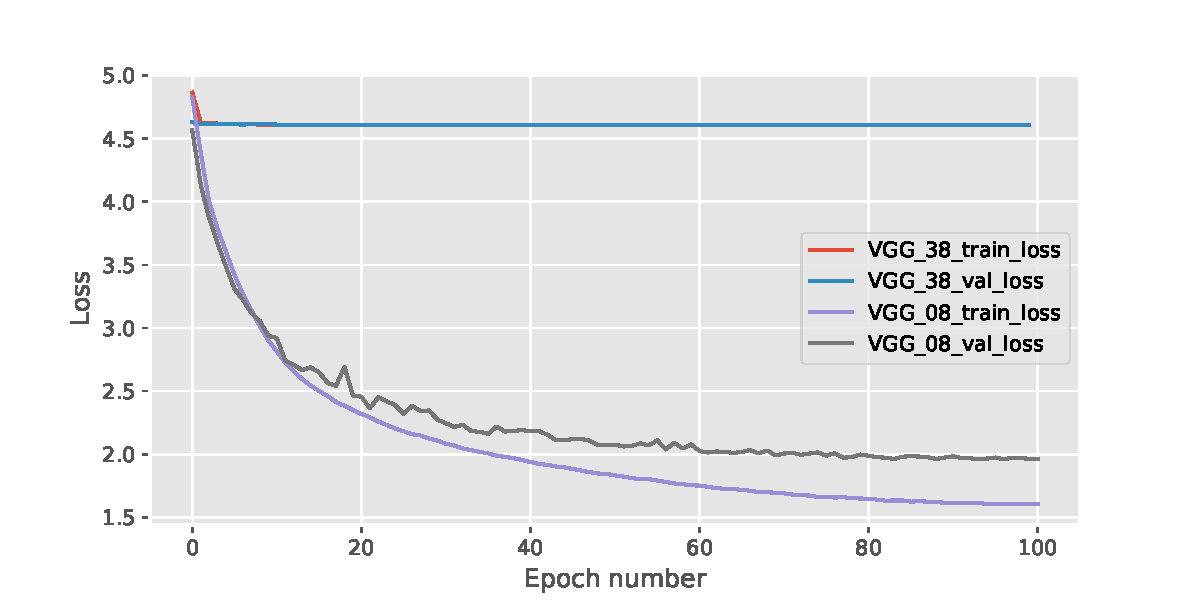
\includegraphics[width=1.1\linewidth]{loss_plot.pdf}
\end{minipage}%
\begin{minipage}{.5\textwidth}
  \centering
  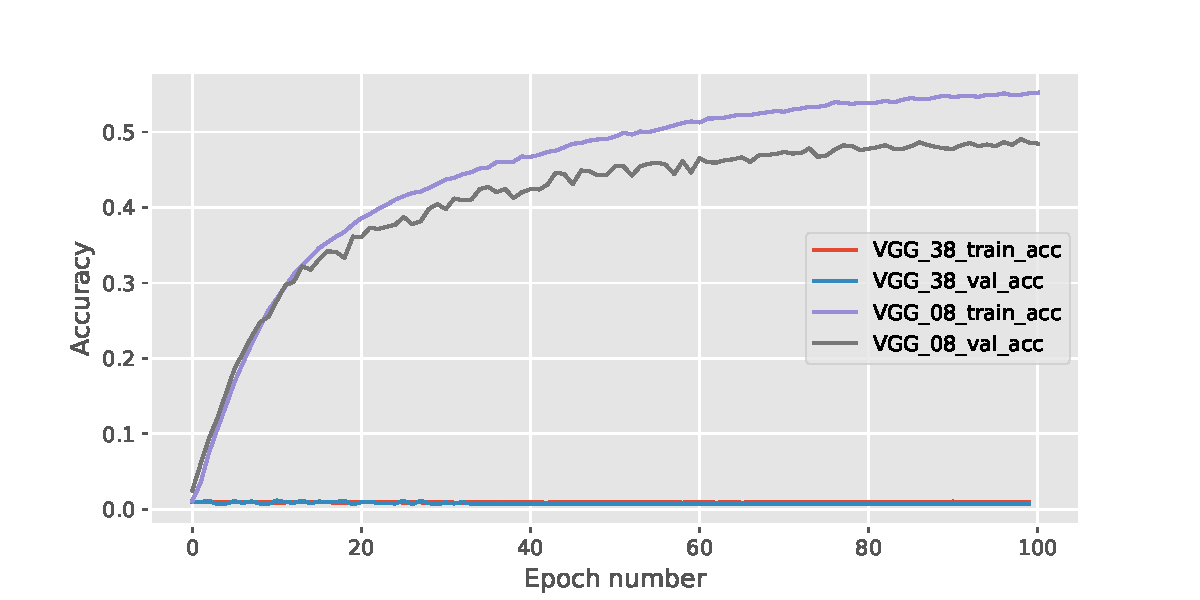
\includegraphics[width=1.1\linewidth]{accuracy_plot.pdf}
\end{minipage}
\caption{Training and validation plots of Healthy (VGG\_08) vs Broken (VGG\_38) in terms of error and accuracy.}
\label{brokenvshealthy}
\end{figure}

\subsection{Introducing our broken CNN}\label{broken-intro}


\textbf{Note: This section's objective is to test your knowledge, understanding and research skill. It's not meant to be an implementation-oriented section. The solutions only require you to add at most 4-5 lines of code.}

Using the Pytorch-based research framework that can be found in the \texttt{pytorch\_mlp\_framework} folder, we have built, trained and evaluated 2 deep CNNs. One consisting of a total of 7 convolutional layers + one fully connected, and another consisting of 37 convolutional layers + one fully connected layer. Figure \ref{brokenvshealthy} illustrates the training/val loss performance of the two models. One can clearly see that the 37 layer CNN (VGG\_38) was unable to minimize its loss, unlike the healthy 7 layer CNN (VGG\_08) which converges to a low error. Given that we know that extra layers means more abstraction power, parameters and capacity, one would expect the deeper model to be doing better at learning than the shallow one, however this is simply not the case. 


\textbf{Identifying the problem}. Construct a hypothesis as to what is causing the issue in Figure \ref{brokenvshealthy}. You can reproduce the figures by running the \texttt{notebooks/Plot\_Results.ipynb} notebook. This file takes as input the collected metrics in folders \texttt{VGG\_08} and \texttt{VGG\_38}.

\textbf{Quantitative Analysis of the problem}. Support your position of the problem using arguments based on quantitative observations. For instance, Figure \ref{fig:healthygradient} shows how the gradient flows in the healthy network, \texttt{VGG\_08} across layers. These are the \textit{gradients with respect to the weights} of the model. Visualize and discuss how gradient flows for the broken network affects/does not affect the loss curves, training and convergence of the 37 layer CNN.  




\begin{figure}
\centering
  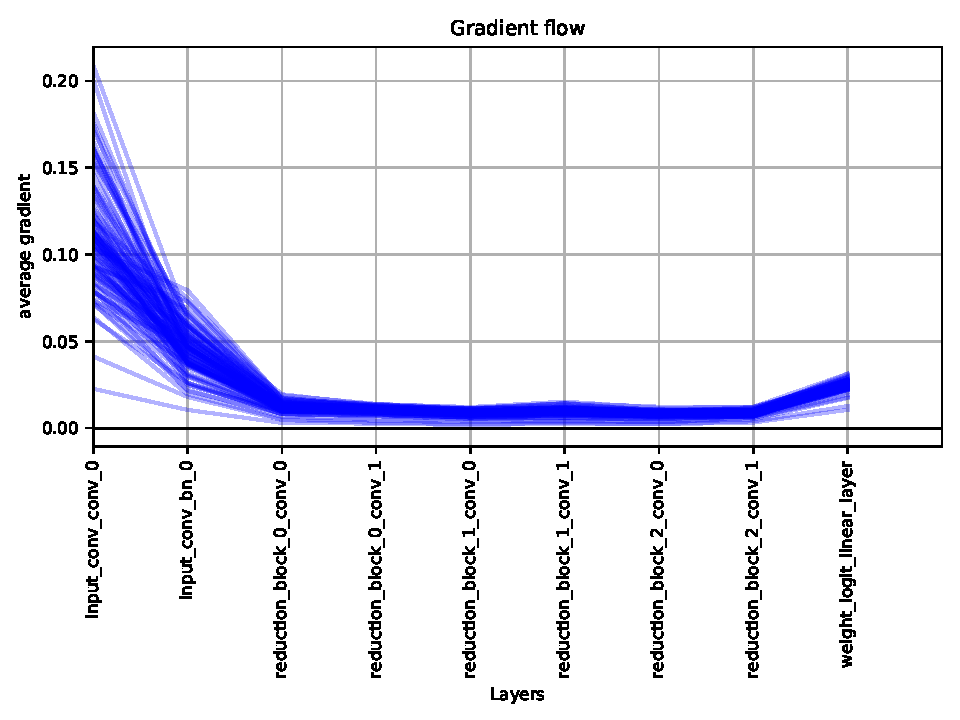
\includegraphics[width=0.8\linewidth]{grad_flow_vgg08.pdf}

\caption{Gradient Flow in each layer for the VGG\_08 network.}
\label{fig:healthygradient}
\end{figure}

\subsubsection{Implementation Guidelines}\label{block-implementation-notes}

The curves shown in Figure \ref{brokenvshealthy} can be reproduced by running the bash scripts to train each model from scratch with the default settings given in \texttt{run\_vgg\_08\_default.sh} and \texttt{run\_vgg\_38\_default.sh}. 

For reproducing Figure \ref{fig:healthygradient} and visualizing the gradient flows for the broken network, implement the function \texttt{plot\_grad\_flows()} within \texttt{pytorch\_mlp\_framework/experiment\_builder.py}. This function takes as input the \texttt{model} parameters during training, accumulates the absolute mean of the gradients in \texttt{all\_grads} and the layer names in \texttt{layers}. The \texttt{matplotlib} function \texttt{plt} plots gradient values for each layer and the function \texttt{plot\_grad\_flows()} returns this final plot.

\emph{(20 Marks)}



\section{Task 2: Background Literature}
\label{sec.related}
\textit{Time budget{\cref{footnote:time-budget}}: This section should take about 20\% of the time you have allocated for your coursework.}\newline

There exist \emph{at least} several methods that can improve the training performance of the broken 37 layer CNN introduced in Section \ref{broken-intro}. Discuss, in your own words and in no \textbf{{any three out of the four research papers}} given below. 

\begin{itemize} 
    \item Batch normalization: Accelerating deep network training by reducing internal covariate shift, \cite{ioffe2015batch}.
    \item Deep residual learning for image recognition, \cite{he2016deep}.
    \item Densely connected convolutional networks, \cite{huang2017densely}
    \item Deeply-supervised nets, \cite{lee2015deeply}
\end{itemize}

This discussion should outline what problems the papers address, are these related to the problem you analyze in Task 1, what/which methods they adopt to solve it, brief details of the method and the final conclusion from the papers. Summary of each paper should be limited to 200-300 words. 

\emph{(20 Marks)}

\section{Task 3: Solution and Experiments}
\textit{Time budget{\cref{footnote:time-budget}}: This section should take about 30\% of the time you have allocated for your coursework.}\newline

\textbf{Solution Overview. }The recommended solutions are in the four papers listed in \cref{sec.related}. Pick and discuss any one solution in detail in this section. Discuss theoretically and intuitively why you chose this solution and how it addresses/improves the training performance of the VGG\_38 model. 


% \cite{ioffe2015batch, he2016deep}. You can also find alternative ones in \cite{huang2017densely, lee2015deeply} which can be more challenging to implement.
\textbf{Experiments. } The recommended solutions are described in \cite{ioffe2015batch, he2016deep}. You can also find alternative ones in \cite{huang2017densely, lee2015deeply} which can be more challenging to implement. We have written the MLP Pytorch framework in a way that allows you to implement said solutions with minimal effort. Each solution will require at approximately 8-10 lines of code. 

\textbf{Important Components to Note}

\begin{enumerate}
    \item The classes \texttt{ConvolutionalProcessingBlock} and \texttt{ConvolutionalDimensionalityReductionBlock} located within \texttt{pytorch\_mlp\_framework/model\_architectures.py}. The former class implements a basic cascade of 2 convolutional layers, each followed by a Leaky ReLU activation function, while the latter implements a basic cascade of 2 convolutional layers, with an average pooling layer in the middle, which effectively halves the height and width dimensions of the tensor volume passing through it. The former is used as the basic building block of the model (repeated \texttt{num\_blocks\_per\_stage times}), while the latter is used only as a dimensionality reduction layer, usually once after each \emph{network stage}. A network stage is considered a cascade of convolutional layers, followed by a dimensionality reduction function such as average pooling. 
    \item Lines 43-50 in \texttt{pytorch\_mlp\_framework/train\_evaluate\_image\_classification\_system.py} showcase how one can create an if-else structure that can read arguments from the command line in order to choose which processing and dim\_reduction blocks will be used.
    \item Lines 17-27 in the same file showcase how some simple data-augmentation strategies can be applied to the system (useful in improving the generalization of the model.)
     
\end{enumerate}

\textbf{Implementing a proposed solution}

\begin{enumerate}
    \item Copy the classes \texttt{ConvolutionalProcessingBlock} and \texttt{ConvolutionalDimensionalityReductionBlock} located within \texttt{pytorch\_mlp\_framework/model\_architectures.py}, and provide a name referring to your proposed solution. Then change the two blocks to implement your proposed solution.
    \item To create a new block ensure that you rewrite the \texttt{build\_module()} and \texttt{forward()} methods.
    \item Add a new clause in the if-else structure in lines 43-50 of  \texttt{pytorch\_mlp\_framework/train\_evaluate} \texttt{\_image\_classification\_system.py} to add a choice for a configuration using your new blocks.
    \item Write small unit-tests for your blocks to ensure that the layers can fprop some data without throwing errors related to Pytorch.
    \item Once tested, you can use the argument parser to easily run experiments with your new modules. Hint: Have a look at the \texttt{block\_type} argument under \texttt{pytorch\_mlp\_framework/arg\_extractor.py}, to get an idea on how to easily pass module names as an argument.
\end{enumerate}

\textbf{Note: Some potential solutions might not require modification of the above, but those are considered more advanced. If you choose that path, you will also bear the responsibility of figuring out the design of your code. That being said, most of known methods can be implemented using the above 3 steps.}

To break this down:

\begin{enumerate}
    \item Select and implement one method to address the problem in Task 1.
    \item Design and run experiments to investigate the performance of the method. Make sure to run your experiments on multiple seeds. 
    \item Build a final model using the knowledge you have gained and evaluate its test performance.
    \item Quantitatively and intuitively analyze how this solution addressed the problem. 
    \item Write about what you did and why in your report.
\end{enumerate}


Important thing to note about experiments:
\begin{enumerate}
    \item The purpose of these experiments is NOT to report results with the best combination of hyper-parameters but finding the ones so that your solution addresses the problem discussed in Task 1 effectively. You will have to do a valid hyper-parameter search over learning rates, batch size, weight decay coefficients, etc. such that your model achieves a stable training and testing accuracy with the proposed solution. Make sure you choose the values wisely and not exhaust your google cloud credits. 
    \item Designing experiments so that you are in a position to draw conclusions from your experiments is more important than doing as many experiments as possible.
    \item When reporting the results of experiments, make sure that the comparison/contrast you are exploring is clear in the way you present the results.
\end{enumerate}

When writing the report on this task you should include the following:
\begin{itemize}
    \item Outline and explain the research questions you are investigating.  Provide citations if appropriate.
    \item Explain the methodology used -- in this case the approach/method picked to solve the problem. Provide citations if appropriate.
    \item Describe carefully the experiments carried out, providing enough information to make them reproducible.  Present your results clearly and concisely.  Graphs and tables should be constructed to make clear the contrasts and comparisons you are interested in based on the research questions. For instance, some interesting evaluation criteria that can be used to compare different strategies are classification accuracy, learning speed of your network and gradients.
    \item Discuss your results, with reference to the research questions, and if appropriate with reference to the literature.  What conclusions can you draw from your experiments and are they consistent with the literature?
\end{itemize}



\subsubsection*{Using Google Compute Engine}
\begin{enumerate}
    \item You will receive an email containing the URL you will need to access in order to request a Google Cloud Platform coupon, and information about how to do this.
    \item In the \texttt{coursework\_2} branch of the GitHub, \texttt{notes/google\_cloud\_setup.md} gives the instructions you should follow to set up a Google Compute Engine instance to carry out this coursework.
    \item The PyTorch experimental framework that is used for this coursework is described in\\\texttt{notes/pytorch-experiment-framework.md} and in\\\texttt{notebooks/Coursework\_2\_Pytorch\_experiment\_framework.ipynb}
\end{enumerate}

\emph{(35 Marks)}

\section{Report}
\label{sec:report}

\textit{Time budget{\cref{footnote:time-budget}}: This section should take about 30\% of the time you have allocated for your coursework.}\newline


Your coursework will be primarily assessed based on your submitted report.

The report template is divided into sections which corresponds to each task in the coursework specs. In addition to the mark distribution for tasks, remaining sections of the report will be graded as follows: \\
\textbf{Abstract and Introduction}: \emph{10 Marks}\\
\textbf{Discussion and Conclusion}: \emph{15 Marks}



The directory \verb+coursework_2/report+ contains a template for your report (\verb+mlp-cw2-template.tex+);  the generated pdf file (\verb+mlp-cw2-template.pdf+) is also provided, and you should read this file carefully as it contains some useful information about the required structure and content. The template is written in LaTeX, and we strongly recommend that you write your own report using LaTeX, using the supplied document style \verb+mlp2020+ (as in the template).

You should copy the files in the \verb+report+ directory to the directory containing the LaTeX file of your report, as \verb+pdflatex+ will need to access these files when building the pdf document from the LaTeX source file. The  \href{https://github.com/VICO-UoE/mlpractical/blob/mlp2020-21/coursework_1/spec/mlp_cw1_2020_21.pdf}{coursework 1 spec} outlines how to create a pdf file from a LaTeX source file.

Your report should be in a 2-column format, based on the document format used for the ICML conference. The report should be a \textbf{maximum of \pagelimit pages long}, not counting the references.  We will not read or assess any parts of the report beyond this limit.

As discussed in the \href{https://github.com/VICO-UoE/mlpractical/blob/mlp2020-21/coursework_1/spec/mlp_cw1_2020_21.pdf}{coursework 1 spec},  all figures should ideally be included in your report file as vector graphics files, rather than raster files as this will make sure all detail in the plot is visible.

% Matplotlib supports saving high quality figures in a wide range of
% common image formats using the
% \href{http://matplotlib.org/api/pyplot_api.html\#matplotlib.pyplot.savefig}{\texttt{savefig}}
% function. \textbf{You should use \texttt{savefig} rather than copying
% the screen-resolution raster images outputted in the notebook.} An
% example of using \texttt{savefig} to save a figure as a PDF file (which
% can be included as graphics in
% \href{https://en.wikibooks.org/wiki/LaTeX/Importing_Graphics}{LaTeX}
% compiled with \texttt{pdflatex} 
% %and in Apple Pages and \href{https://support.office.com/en-us/article/Add-a-PDF-to-your-Office-file-74819342-8f00-4ab4-bcbe-0f3df15ab0dc}{Microsoft Word} documents)
% is given below.

% \begin{Shaded}
% \begin{Highlighting}[]
% \CharTok{import} \NormalTok{matplotlib.pyplot }\CharTok{as} \NormalTok{plt}
% \CharTok{import} \NormalTok{numpy }\CharTok{as} \NormalTok{np}
% \CommentTok{# Generate some example data to plot}
% \NormalTok{x = np.linspace(}\DecValTok{0}\NormalTok{., }\DecValTok{1}\NormalTok{., }\DecValTok{100}\NormalTok{)}
% \NormalTok{y1 = np.sin(}\DecValTok{2}\NormalTok{. * np.pi * x)}
% \NormalTok{y2 = np.cos(}\DecValTok{2}\NormalTok{. * np.pi * x)}
% \NormalTok{fig_size = (}\DecValTok{6}\NormalTok{, }\DecValTok{3}\NormalTok{)  }\CommentTok{# Set figure size in inches (width, height)}
% \NormalTok{fig = plt.figure(figsize=fig_size)  }\CommentTok{# Create a new figure object}
% \NormalTok{ax = fig.add_subplot(}\DecValTok{1}\NormalTok{, }\DecValTok{1}\NormalTok{, }\DecValTok{1}\NormalTok{)  }\CommentTok{# Add a single axes to the figure}
% \CommentTok{# Plot lines giving each a label for the legend and setting line width to 2}
% \NormalTok{ax.plot(x, y1, linewidth=}\DecValTok{2}\NormalTok{, label=}\StringTok{'$y = \textbackslash{}sin(2\textbackslash{}pi x)$'}\NormalTok{)}
% \NormalTok{ax.plot(x, y2, linewidth=}\DecValTok{2}\NormalTok{, label=}\StringTok{'$y = \textbackslash{}cos(2\textbackslash{}pi x)$'}\NormalTok{)}
% \CommentTok{# Set the axes labels. Can use LaTeX in labels within $...$ delimiters.}
% \NormalTok{ax.set_xlabel(}\StringTok{'$x$'}\NormalTok{, fontsize=}\DecValTok{12}\NormalTok{)}
% \NormalTok{ax.set_ylabel(}\StringTok{'$y$'}\NormalTok{, fontsize=}\DecValTok{12}\NormalTok{)}
% \NormalTok{ax.grid(}\StringTok{'on'}\NormalTok{)  }\CommentTok{# Turn axes grid on}
% \NormalTok{ax.legend(loc=}\StringTok{'best'}\NormalTok{, fontsize=}\DecValTok{11}\NormalTok{)  }\CommentTok{# Add a legend}
% \NormalTok{fig.tight_layout()  }\CommentTok{# This minimises whitespace around the axes.}
% \NormalTok{fig.savefig(}\StringTok{'file-name.pdf'}\NormalTok{) }\CommentTok{# Save figure to current directory in PDF format}
% \end{Highlighting}
% \end{Shaded}


If you make use of any any books, articles, web pages or other resources
you should appropriately cite these in your report. You do not need to
cite material from the course lecture slides or lab notebooks.



% To create a pdf file \verb+mlp-cw2-template.pdf+ from a LaTeX source file (\verb+mlp-cw2-template.tex+), you can run the following in a terminal:
% \begin{verbatim}
% pdflatex mlp-cw2-template
% bibtex mlp-cw2-template
% pdflatex mlp-cw2-template
% pdflatex mlp-cw2-template
% \end{verbatim}
% (Yes, you have to run pdflatex multiple times, in order  for latex to construct the internal document references.)

% An alternative, simpler approach uses the \verb+latexmk+ program:
% \begin{verbatim}
% latexmk -pdf mlp-cw2-template
% \end{verbatim}

% Another alternative is to use an online LaTeX authoring environment such as \url{https://overleaf.com} -- note that all staff and students have free access to Overleaf Pro - see \url{https://www.ed.ac.uk/information-services/computing/desktop-personal/software/main-software-deals/other-software/overleaf}.

% It is worth learning how to use LaTeX effectively, as it is particularly powerful for mathematical and academic writing.  There are many tutorials on the web.


\section{Mechanics}
\label{sec:mechanics}

\textbf{Marks:} 
This assignment will be assessed out of 100 marks and forms \markweight\% of your final grade for the course.

\textbf{Academic conduct:} 
Assessed work is subject to University
regulations on academic
conduct:\\ {\small \url{http://web.inf.ed.ac.uk/infweb/admin/policies/academic-misconduct}}

\textbf{Submission:} 
You can submit more than once up until the submission deadline. All
submissions are timestamped automatically. Identically named files
will overwrite earlier submitted versions, so we will mark the latest
submission that comes in before the deadline.

If you submit anything before the deadline, you may not resubmit
after the deadline. (This policy allows us to begin marking submissions
immediately after the deadline, without having to worry that some may
need to be re-marked).

If you do not submit anything before the deadline, you may submit {\em
exactly once} after the deadline, and a late penalty will be applied
to this submission unless you have received an approved extension.
Please be aware that late submissions may receive lower priority for
marking, and marks may not be returned within the same timeframe as
for on-time submissions.

{\em Warning:} Unfortunately the submission system on Learn will technically
allow you to submit late even if you submitted before the deadline
(i.e.\ it does not enforce the above policy). Don't do this! We will
mark the version that we retrieve just after the deadline.

\textbf{Extension requests:} 
For additional information about late penalties and extension
requests, see the School web page below. \textbf{Do  not email any course
staff directly about extension requests as these are handled by the ITO; 
you must follow the instructions on the web page.}

{\small \url{http://web.inf.ed.ac.uk/infweb/student-services/ito/admin/coursework-projects/late-coursework-extension-requests}}

\textbf{Late submission penalty:}  
Following the University guidelines, 
late coursework submitted without an authorised extension will be
recorded as late and the following penalties will apply: 5
percentage points will be deducted for every calendar day or part
thereof it is late, up to a maximum of 7 calendar days. After this
time a mark of zero will be recorded.

\subsection{Backing up your work}
\label{sec:backing-up-your-work}

It is \textbf{strongly recommended} you use some method for backing up
your work. Those working in their AFS homespace on DICE will have their
work automatically backed up as part of the
\href{http://computing.help.inf.ed.ac.uk/backups-and-mirrors}{routine
backup} of all user homespaces. If you are working on a personal
computer you should have your own backup method in place (e.g.~saving
additional copies to an external drive, syncing to a cloud service or
pushing commits to your local Git repository to a private repository on
Github). \textbf{Loss of work through failure to back up
\href{http://web.inf.ed.ac.uk/infweb/student-services/ito/admin/coursework-projects/late-coursework-extension-requests}{does not constitute a good reason for
late submission}}.

You may \emph{additionally} wish to keep your coursework under version
control in your local Git repository on the \verb+coursework_2+ branch.

If you make regular commits of your work on the coursework this will
allow you to better keep track of the changes you have made and if
necessary revert to previous versions of files and/or restore
accidentally deleted work. This is not however required and you should
note that keeping your work under version control is a distinct issue
from backing up to guard against hard drive failure. If you are working
on a personal computer you should still keep an additional back up of
your work as described above.


\subsection{Submission}
\label{sec:submission}

Your coursework submission should be done online on the \href{https://www.learn.ed.ac.uk/}{Learn} course webpage.

Your submission should include one zip file \texttt{sxxxxxxx.zip} that should contain a folder named sxxxxxxx. This folder should have - 

\begin{itemize}

  %generated for part 1, \verb+sXXXXXXX_batchnorm_test_file.txt+ and\\ \verb+sXXXXXXX_conv_test_file.txt+, where your student number replaces \verb+sXXXXXXX+.  Please do not   change the names of these files.

\item
  your completed report as a PDF file renamed as \texttt{sxxxxxxx\_report.pdf}, using the provided template
  
\item your local version of the Pytorch experiment framework (\texttt{mlp/pytorch\_experiment\_scripts}), including any changes you've made to existing files and any newly created files.
\item a copy of your Pytorch experiment directories (\texttt{mlp/results}), including \textbf{only} the \texttt{.csv} files for your training, validation and test statistics. Please do not include model weights.

\end{itemize}
Please do not submit anything else (e.g. log files).

You should copy all of the files to a single directory, \verb+sxxxxxxx+, e.g.

Your folder directory structure should look like this - 
\dirtree{%
.1 sxxxxxxx.
.2 sxxxxxxx\_report.pdf.
.2 mlp.
.3 \texttt{pytorch\_experiment\_scripts/}.
.3 \texttt{results/}.
}



You can use this command on Linux machines to zip all the files together - 

\texttt{zip sxxxxxxx.zip  sxxxxxxx}

Replace \texttt{sxxxxxxx} with your student id. 

Once you have successfully created the .zip file, you need to login to your Learn \texttt{Machine Learning Practical (2020-2021)[YR]} webpage and submit the file. 
\begin{itemize}
    \item Migrate to the section \textbf{Coursework} on the left column on the course page. 
    \item Click on Coursework 2.
    \item A page will appear where you will need to browse and upload your .zip file that you created previously in \texttt{Attach Files} and then click \textbf{Submit}. 
\end{itemize}

You can amend an existing submission by attaching a different .zip file using the Attach Files option and then Submit again.

\textbf{Note that we will only mark the last uploaded coursework in case you amend your files. Thus it is your responsibility to make sure that correct files are uploaded.}



\section{Marking Guidelines}
\label{sec:marking-scheme}
This document (Section \ref{sec:tasks} in particular) and the template report (\verb+mlp-cw2-template.pdf+) provide a description of what you are expected to do in this assignment, and how the report should be written and structured.

Assignments will be marked using the scale defined by the \textbf{University Common Marking Scheme}:
\begin{center}
\begin{tabular}{lll}
Numeric mark & Equivalent letter grade & Approximate meaning \\
$< 40$ & F & fail \\
40-49 & D & poor \\
50-59 & C & acceptable \\
60-69 & B & good \\
70-79 & A3 & very good/distinction \\
80-100 & A1, A2 & excellent/outstanding/high distinction
\end{tabular}
\end{center}

Please note the University specifications for marks above 50:

{\bf A1 90-100}
Often faultless. The work is well beyond what is expected for the level of study.

{\bf A2 80-89}
A truly professional piece of scholarship, often with an absence of errors. \\
As `A3' but shows (depending upon the item of assessment):
significant personal insight / creativity / originality
and / or
extra depth and academic maturity in the elements of assessment.

{\bf A3 70-79}\\
\emph{Knowledge}: Comprehensive range of up-to-date material handled in a professional way.\\
\emph{Understanding/handling of key concepts}: Shows a command of the subject and current theory.\\
\emph{Focus on the subject}: Clear and analytical; fully explores the subject.\\
\emph{Critical analysis and discussion}: Shows evidence of serious thought in critically evaluating and integrating the evidenced and ideas. Deals confidently with the complexities and subtleties of the arguments. Shows elements of personal insight / creativity / originality.\\
\emph{Structure}: Clear and coherent showing logical, ordered thought.\\
\emph{Presentation}: Clear and professional with few, relatively minor flaws. Accurate referencing. Figures and tables well constructed and accurate. Good standard of spelling and grammar.



{\bf B 60-69} \\
\emph{Knowledge}: Very good range of up-to-date material, perhaps with some gaps, handled in a competent way.\\
\emph{Understanding and handling of key concepts}: Shows a firm grasp of the subject and current theory but there may be gaps.\\
\emph{Focus on the subject}: Clear focus on the subject with no or only trivial deviation.\\
\emph{Critical analysis and discussion}: Shows initiative, the ability to think clearly, critically evaluate ideas, to bring different ideas together, and to draw sound conclusions.\\
\emph{Structure}: Clear and coherent showing logical, ordered thought. Additionally for code: re-usability may be somewhat limited. No unused variables or dead code.\\
\emph{Presentation}: Clear and well presented with few, relatively minor flaws. For writing: Accurate referencing; using the correct referencing system. Figures and tables well-constructed and accurate. Good standard of spelling and grammar. Alternatively for code: well-documented, readable code.\\



{\bf C 50-59} \\
\emph{Knowledge}: Sound but limited. Inaccuracies, if any, are minor.\\
\emph{Understanding and handling of key concepts}: Understands the subject but does not have a firm grasp and depth of understanding of all the key concepts.\\
\emph{Focus on the subject}: Addresses the subject with relatively little irrelevant material.\\
\emph{Critical analysis and discussion}: Limited critical analysis and evaluation of sources of evidence.\\
\emph{Structure}: Reasonably clear and coherent, generally structuring ideas and information or code in a logical way. Additionally for code: Few or no unused variables or dead code.\\
\emph{Presentation}: Generally well presented but there may be some flaws, for example in figures, tables, referencing technique and standard of English. Alternatively for code: generally well-documented, readable code, but with some weaknesses.\\




\bibliographystyle{plainnat}
\bibliography{mlp-cw-references}
\end{document}
